In this chapter we present the design principles of a PREcision Timed (PRET) Machine.
Specifically, we discuss the implementation of a predictable pipeline and memory controller, and present timing extensions to the ISA. 
It is important to understand why and how current architectures fall short of timing predictability and repeatability.
Thus, we first discuss the common architectural designs and their effects on execution time, and point out some key issues and tradeoffs when designing architectures for predictable and repeatable timing.

\section{Pipelines}
The introduction of pipelining vastly improves the performance of processors.
Pipelining increases the number of instructions that can be processed at one time by splitting up instruction execution into multiple steps.
It allows for faster clock speeds, and improves instruction throughput compared to single cycle architectures.
Ideally in each processor cycle, one instruction completes and leaves the pipeline as another enters and begins execution. 
In reality, different pipeline hazards occur that reduce the throughput and create stalls in the pipeline.
The techniques introduced to mitigate the penalties of pipeline hazards greatly effect to the timing predictability and repeatability of architectures.     
We analyze several commonly used techniques to reduce the performance penalty from hazards, and show their effects on execution time and predictability. 

\subsection{Pipeline Hazards}
\label{sec:pipeline_hazards}
\subsubsection{Data Hazards}

\begin{wrapfigure}{r}{0.5\textwidth}
  \vspace{-30pt}
  \begin{center}
    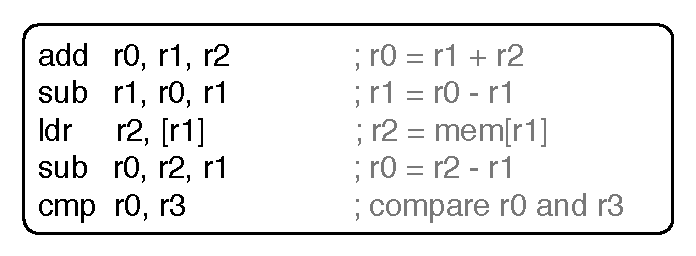
\includegraphics[scale=.65]{figs/sample_data_dependent_code}
  \end{center}
  \vspace{-3mm}
  \caption{Sample code with data dependencies}
  \label{fig:sample_data_dependent_code}
\end{wrapfigure}

Data hazards occur when the data needed by an instruction are not yet available.
Pipelines begin the execution of instructions before preceding ones are finished.
Thus, consecutive instructions that are data-dependent can simultaneously be executing in the pipeline.
For example, the code in figure~\ref{fig:sample_data_dependent_code} shows assembly instructions from the ARM instruction set architecture (ISA).
Each instruction in the code segment depends on the result of its previous instruction.
Figure~\ref{fig:data_depend_execution_non_interleaved} shows two ways data hazards are commonly handled in pipelines. 

\begin{figure}
\vspace{-20pt} 
\begin{center}
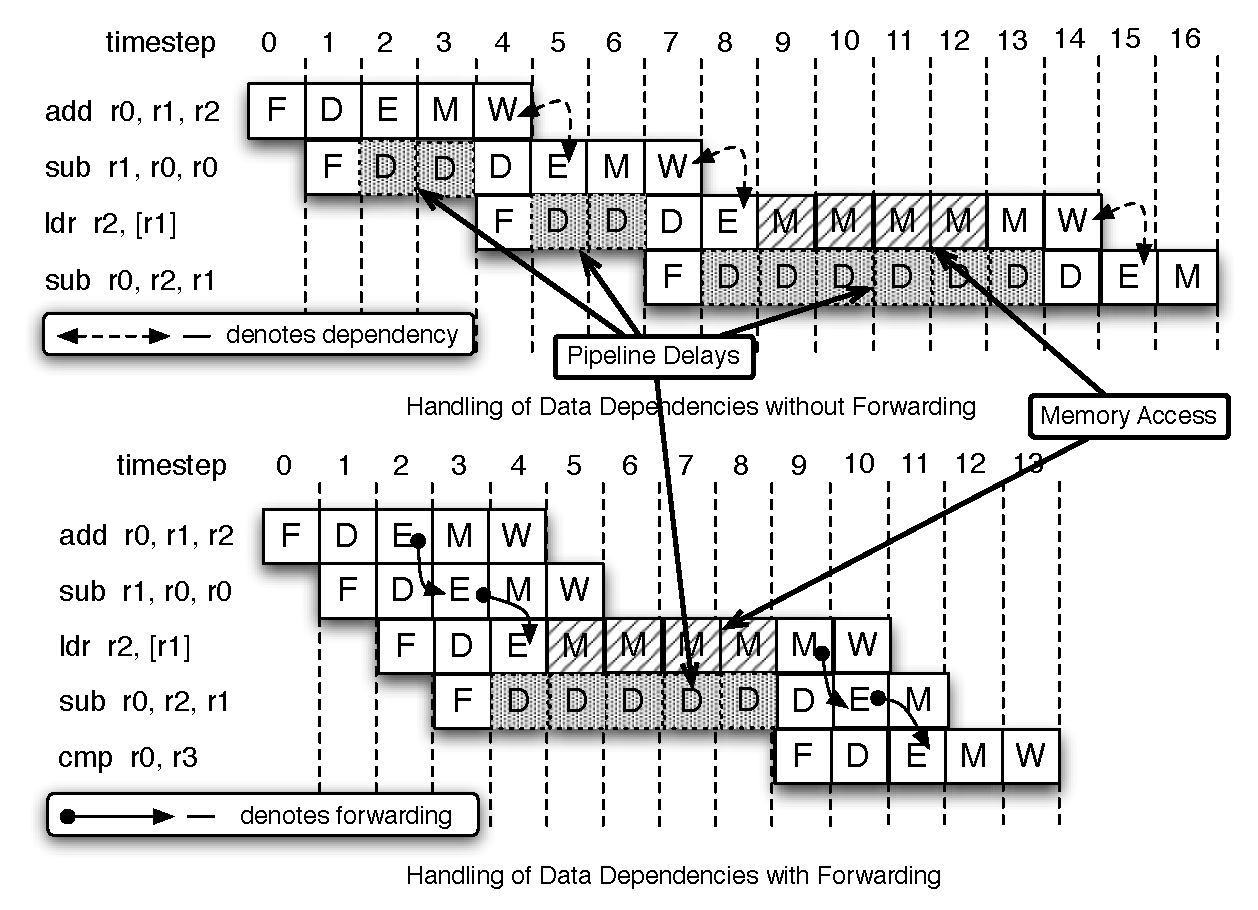
\includegraphics[scale=.6]{figs/data_depend_execution_non_interleaved}
\end{center}
\vspace{-3mm}
\caption{Handling of data dependencies in single threaded pipelines}
\label{fig:data_depend_execution_non_interleaved}
\end{figure}

In the figure, time progresses horizontally towards the right.
Each column represents a processor cycle.
Each row represents an instruction that is fetched and executed within the pipeline.
Each block represents the instruction entering the different stages of the pipeline -- fetch (F), decode (D), execute (E), memory (M) and writeback (W).   
We assume a classic five stage RISC pipeline.

A simple but effective technique stalls the pipeline until the previous instruction completes.
This is shown in the top of figure~\ref{fig:data_depend_execution_non_interleaved}, as delays are inserted to wait for the results from previous instructions.
The dependencies between instructions are explicitly shown in the figure to make clear why the pipeline delays are necessary.
The performance penalty incurred in this case comes from the pipeline delays inserted.

\emph{Data forwarding} is commonly used to mitigate the delays when data hazards occur.
Pipelines split up the execution of instructions into different execution stages. 
Thus, the results from an instruction could be ready, but waiting to be committed in the last stage of the pipeline.
Data forwarding introduces backwards data paths in the pipeline, so earlier pipeline stages can access the data from instructions in later stages that have not yet committed.
This greatly reduces the delays inserted in the pipeline.
The circuitry for data forwarding usually consists of the backwards data paths and multiplexers in the earlier pipeline stages to select the correct data to be used.    
The pipeline controller dynamically detects whether a data dependency exists, and changes the selection bits of the multiplexers accordingly.

The bottom of figure~\ref{fig:data_depend_execution_non_interleaved} shows the execution sequence of the previous example in a pipeline with data forwarding.
No pipeline delays are inserted for the first \emph{sub} and \emph{ldr} instruction because the data they depend on are forwarded.
However, delays are still inserted for the second \emph{sub} instruction after the \emph{ld} instruction.
For longer latency operations, such as memory accesses, the results are not yet available to be forwarded by the forwarding paths, so pipeline delays are still required. 
This illustrates the limitations of data forwarding.
They can address data hazards that result from pipelining, such as read-after-write register operations, but they cannot address data hazards that result from long latency operations, such as memory operations.
More involved techniques such as the out-of-order execution or superscalars are required to mitigate the effects of long latency operations.

The handling of data hazards in pipelines can cause instructions to exhibit dynamic execution times.  
For example, figure~\ref{fig:data_depend_execution_non_interleaved} shows the \emph{sub} instruction, in both top and bottom figures, exhibiting different execution times. 
To determine the execution time of instructions on pipelines that stall for data hazards, we need to determine when a stall is inserted, and how long the pipeline is stalled for.
Stalls are required when the current instruction uses the results of a previous instruction that is still in execution in the pipeline.
Thus, depending on the pipeline depth, a window of previous instructions needs to be checked to determine whether any stalls are inserted.     
The length of the stall is determined by the execution time of the dependent instructions, because the pipeline will stall until those instructions complete.
Data forwarding does not remove the data hazards, but only reduces the number of stalls required to take care of the data hazards.  
Thus, to determine the execution time when data forwarding is used, timing analysis needs to determine when the data forwarding circuitry cannot not forward the data for data hazards.
%This can similarly be done by observing the window of instructions not yet committed in the pipeline.  
%The difference is, instead of all data dependencies, only data dependencies from long latency operations need to be detected.

Both stalling and forwarding cause the execution time of instructions to depend on a window of previous instructions.
The deeper the pipeline, the larger the window.
Thus, execution time analysis needs to model and account for this additional window of instructions on pipelined architectures that use stalling or forwarding to handle the data hazards. 

\subsubsection{Control Hazards}
\begin{wrapfigure}{r}{0.5\textwidth}
  \vspace{-20pt}
  \begin{center}
    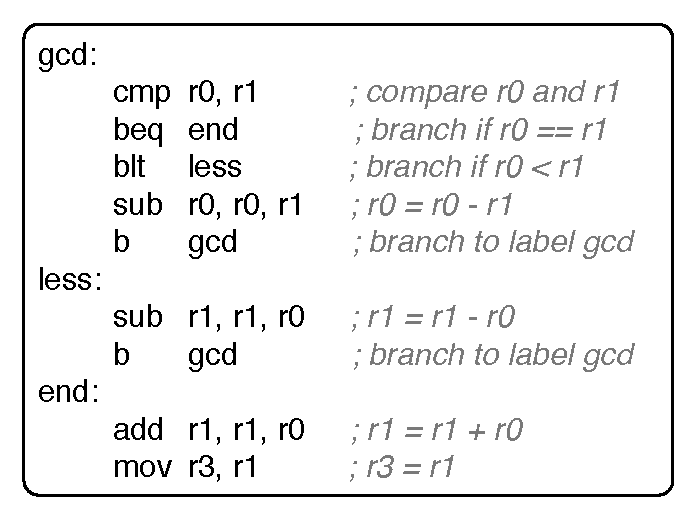
\includegraphics[scale=.65]{figs/sample_gcd_code}
  \end{center}
  \vspace{-3mm}
  \caption{GCD with conditional branches}
  \label{fig:sample_gcd_code}
\end{wrapfigure}

Branches cause control-flow hazards, or control hazards, in the pipeline; the instruction after the branch, which should be fetched the next cycle, is unknown until after the branch instruction is completed.
Conditional branches further complicate matters, as whether or not the branches are taken depends on an additional condition that could also be unknown when the conditional branches are in execution. 
The code segment in figure~\ref{fig:sample_gcd_code} implements the \emph{Greatest Common Divisor} (GCD) algorithm using the conditional branch instructions \emph{beq} (branch equal) and \emph{blt} (branch less than) in the ARM ISA.  
Conditional branch instructions in ARM branch based on conditional bits that are stored in a processor state register.
The conditional bits can be set based on the results of standard arithmetic instructions~\cite{armrefman}.
The \emph{cmp} instruction is one such instruction that subtracts two registers and sets the conditional bits according to the results.
The GCD implementation shown in the code uses this mechanism to determine whether to continue or end the algorithm.
Figure~\ref{fig:branch_execution_non_interleaved_pipeline} shows the execution of the conditional branches from our example, and demonstrates two commonly used techniques to handling control hazards in pipelines. 
To show only the timing effects of handling control hazards, we assume an architecture with data forwarding that handles data hazards.
As there are no long latency instructions in our example, all stalls observed in the figure are caused by the handling of control hazards.  

\begin{figure}
\begin{center}
\noindent\makebox[\textwidth]{%
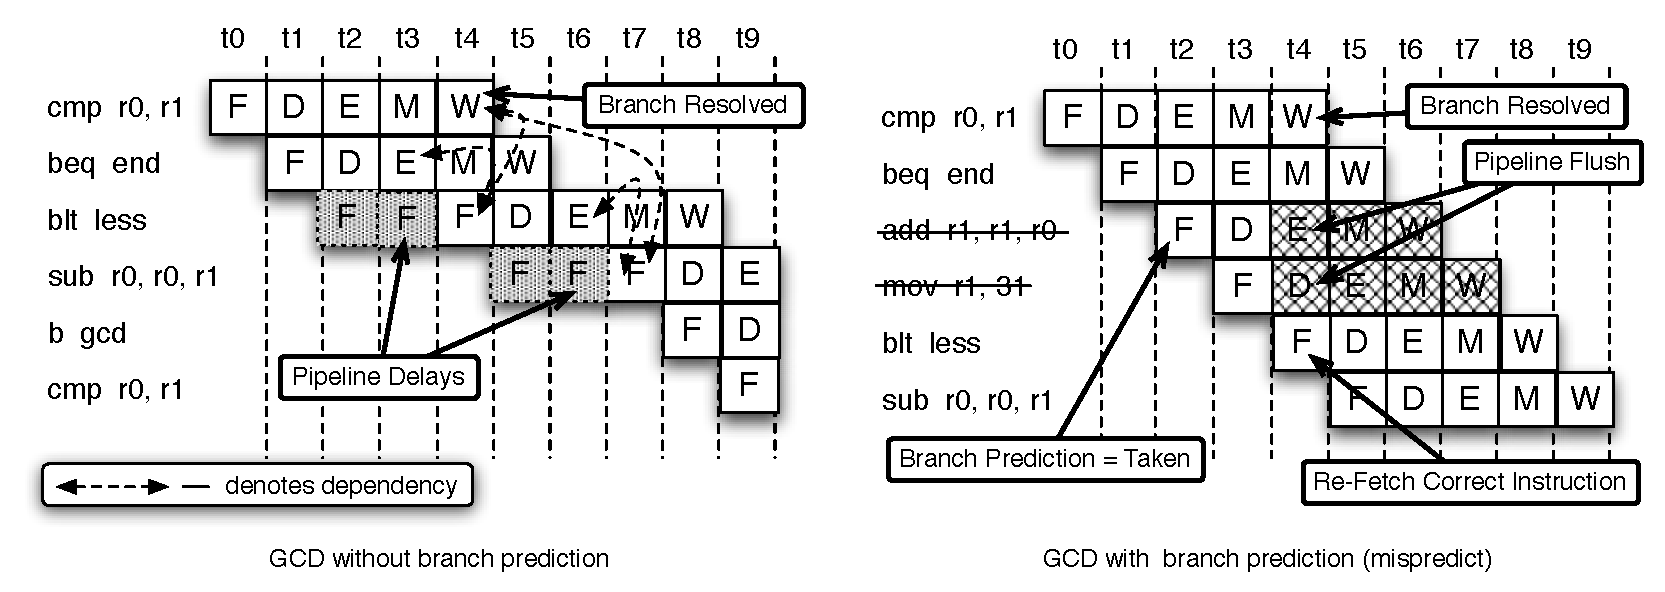
\includegraphics[scale=.58]{figs/branch_execution_non_interleaved_pipeline}}
\end{center}
\vspace{-3mm}
\caption{Handling of conditional branches in single threaded pipelines}
\label{fig:branch_execution_non_interleaved_pipeline}
\end{figure}

Similar to data hazards, control hazards can also be handled by stalling the pipeline until the branch instruction completes. 
This is shown on the left of figure~\ref{fig:branch_execution_non_interleaved_pipeline}. 
%The dependencies between instructions are explicitly shown to make clear why the pipeline delays are necessary.
Branch instructions typically calculate the target address in the execute stage, so two pipeline delays are inserted before the fetching of the \emph{blt} instruction to wait for \emph{beq} to complete the target address calculation. 
The same reasoning applies to the two pipeline delays inserted before the \emph{sub} instruction. 
The performance penalty (often referred to as the \emph{branch penalty}) incurred in this case is the two delays inserted after every branch instruction, to wait for the branch address calculation to complete.

To mitigate the branch penalty, some architectures require the compiler to insert one or more non-dependent instructions after each branch instruction.
These instruction slots are called branch delay slots, and are always executed before the pipeline branches to the target address. 
This way, instead of wasting cycles to wait for the target address calculation, the pipeline continues to execute useful instructions before it branches.
However, if the compiler cannot place useful instructions in the branch delay slot, \emph{nops} need to be inserted into those slots to ensure correct program execution.
Thus, branch delay slots are less effective for deeper pipelines, because more delay slots need to be filled by the compiler to account for the branch penalty.
  
Instead of stalling, \emph{branch predictors} are commonly employed to predict the branch condition and target address so the pipeline can speculatively continue its execution. 
Branch predictors internally maintain a state machine that is used to determine the prediction of each branch.  
The internal state is updated after each branch according to the results of the branch. 
Different prediction schemes have been proposed, and some can even accurately predict branches up to 98.1\%~\cite{Mcfarling_Branch_predict}.  
If the branch prediction is correct, no penalty is incurred for the branch because the correct instructions are speculatively executed.  
%With branch predictor, the pipeline fetches the next instruction based upon the results of the branch prediction, and continues to execute speculatively.
However, when the prediction is incorrect (often referred to as a \emph{branch midpredict}), the speculatively executed instructions are flushed, and the correct instructions are re-fetched into the pipeline for execution.

The right of figure~\ref{fig:branch_execution_non_interleaved_pipeline} shows the execution of GCD in the case of a branch misprediction.
The \emph{beq} branch is predicted to be taken, so the \emph{add} and \emph{mov} instructions from label \emph{end} are directly fetched into execution. 
When \emph{beq} progresses past the execute stage, \emph{cmp} has forwarded its results used to determine the branch condition, and the branch target address has been calculated, so the branch is resolved.
At this point, the misprediction is detected, so the \emph{add} and \emph{mov} instructions are flushed out of the pipeline. 
The next instruction from the correct path, the \emph{blt} instruction, is immediately re-fetched, and execution continues.
The performance penalty of branch mispredictions is derived from the number of pipeline stages between instruction fetch and branch resolution.  
In our example, the misprediction penalty is 2, as branches are resolved after the execute stage.
This penalty only occurs on a branch mispredict, thus branch predictors with high success rates typically improve average performance of pipelines drastically, compared to architectures that simply stall for branches.
%However, for more complex architectures with caches or other hardware states, the effects of incorrectly fetched instructions on the state of the processor less well-known and studied. 

Stalling and branch predicting exhibit vastly different effects on execution time.    
When stalls are used to handle control hazards, the execution time effects are static and predictable.   
The pipeline will simply \emph{always} insert pipeline delays after a branch instruction.
Thus, no extra complexity is added to the execution time analysis; the latency of branch instructions simply needs to be adjusted to include the branch penalty.
On the other hand, if a branch predictor is employed, the execution time of each branch will vary depending on the result of the branch prediction.  
To determine the success of a branch prediction, the prediction and the branch outcome, both of which can dynamically change in run-time, must be known.   
Program path analysis can attempt to analyze the actual outcome of branches statically from the program code. 
However, the predictions made from the branch predictor depend on the internal state stored in the hardware unit.
This internal state, updated by each branch instruction, must be explicitly modeled in order to estimate the prediction. 
If the predictor state is unknown, the miss penalty must conservatively be accounted for.
There has been work on explicitly modeling branch predictors for execution time analysis~\cite{Mitra_branch_wcet_2002}, but the results only take into account the stalls from the branch penalty. 
Caches and other processor states are assumed to be perfect. 
In reality, the speculative execution on the predicted program paths lead to further complications that need to be accounted for.
Other internal states exist in the architecture that could be affected by speculatively executing instructions.
For example, if caches are used, their internal state could be updated during the speculative execution of a mispredicted path.
As architectures grow in complexity, the combined modeling of all hardware states in the architecture often leads to an intractable explosion in state space for the analysis.    
This makes a tight static execution time analysis extremely difficult, if not impossible.

The difference in execution time effects between stalling and employing a branch predictor highlights an important tradeoff for architecture designs.    
It is possible to improve average-case performance by making predictions, and speculatively executing based upon them.
However, this comes at the cost of predictability, and a potential decreasing of the worst-case performance.  
For real-time and safety critical systems, the challenge remains to improve worst-case performance while maintaining predictability, and how pipeline hazards are handled plays a key role in tackling this challenge. 
 
Although less often mentioned, the presence of interrupts and exceptions in the pipeline also creates control hazards. 
Exceptions can occur during the execution of any instruction and change the control flow of the program to execute the exception handler.
For single threaded pipelines, this means that all instructions fetched and not committed in the pipeline are speculative, because when an exception occurs, all uncommitted instructions in the pipeline become invalid.
%Pipelines often handle this by flushing all instructions and fetching the exception handler for execution.      
These effects are acknowledged, but often ignored in static analysis because it is simply impossible to model every possible exception and its effect on the architecture states. 
 
\subsubsection{Structural Hazards}
Structural hazards occur when a processor's hardware component is needed by two or more instructions at the same time. 
For example, a single memory unit accessed both in the fetch and memory stage results in a structural hazard. 
The design of the pipeline plays an integral part in eliminating structural hazards. 
For example, the classic RISC five stage pipeline only issues one instruction at a time, and uses separate instruction and data caches to avoid structural hazards.
Structural hazards are generally much more prevalent in architectures that issue multiple instructions at a time.
If structural hazards cannot be avoided, then the pipeline must stall to enforce sequential access to the contended hardware component.
The execution time effects of structural hazards are specific to how contention is managed for each pipeline design.
Here we omit a general discussion of the timing effects, and later address them specifically for our proposed architecture. 

\subsection{Pipeline Multithreading}
Discussed above, \emph{data forwarding} and \emph{branch prediction} are simple techniques employed to handle pipeline hazards. 
Advanced architectures, such as \emph{superscalar} and \emph{VLIW} machines, employ more complex mechanisms to improve the average performance of the architecture.  
Both architectures issue multiple instructions every cycle, and superscalar machines dynamically execute instructions out-of-order if no dependency is detected.    
These architectures exploit \emph{instruction-level parallelism} to overlap the execution of instructions from a single thread whenever possible.         
On the contrary, \emph{multithreaded architectures} exploit \emph{thread-level parallelism} to overlap the execution of instructions from different hardware threads. 
Each hardware thread in a multithreaded architecture has its own physical copy of a processor state, such as the register file and program counter.
When a pipeline hazard arises from the execution of a hardware thread, another hardware thread can be fetched for execution to avoid stalling the pipeline. 
This improves the instruction throughput of the architecture.

\begin{figure}[h]
\begin{center}
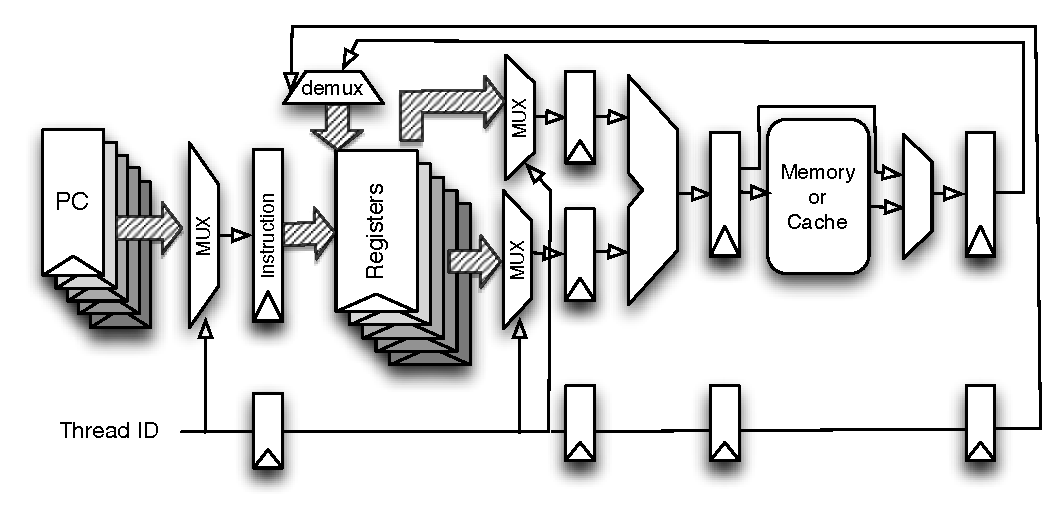
\includegraphics[scale=.8]{figs/multithreaded_pipeline_block}
\end{center}
\vspace{-10pt}
\caption{Simple Multithreaded Pipeline}
\label{fig:multi-thread pipeline simplified}
\end{figure}
Figure~\ref{fig:multi-thread pipeline simplified} shows the implementation of a simple multithreaded pipeline.
It contains 5 hardware threads, so it has 5 copies of the Program Counter (PC) and register files.
The rest of the pipeline remains similar to a classic five stage RISC pipeline, with the addition of a few multiplexers used to select the thread states.
Thus, the extra copies of the processor state and multiplexers are most of the hardware additions needed to implement hardware multithreading.
When a hardware thread executes in the pipeline, its corresponding thread state is passed into the pipeline to be used.
In most of this thesis, the term \emph{threads} refers to the explicit hardware threads that have physical hardware copies of the thread state.
This is not to be confused with the common notion of \emph{threads}, which describes software contexts managed by an operating system, with its states stored in memory.
It will be explicitly noted when we refer to the software notion of threads. 
%The selection of threads for execution is one of the most important factors to fully utilize thread-level parallelism.
%If a thread is stalled waiting for memory access but gets selected to execute in the pipeline, then that instruction slot is wasted and the processor isn't fully utilized.
Ungerer et al.~\cite{Ungerer:2003:survey_multithreading} survey different multithreaded architectures and categorize them based upon the \emph{thread scheduling} policy and the \emph{execution width} of the pipeline.

The \emph{thread scheduling} policy determines which threads are executing, and how often a context switch occurs.  
\emph{Coarse-grain} policies manage threads similarly to the way operation systems manage software threads.
A thread gains access to the pipeline and continues to execute until a context switch is triggered.
Context switches occur less frequently via this policy, so fewer threads are required to fully utilize the processor.
Different coarse-grain policies trigger context switches with different events. 
Some policies trigger context switches on dynamic events, such as a cache miss or an interrupt; some policies trigger context switches on more static events, such as specialized instructions.
\emph{Fine-grain} policies switch context much more frequently -- some as frequently as every processor cycle.
The \emph{execution width} of the pipeline is the number of instructions fetched each cycle.  
Multithreaded architectures with wider pipeline widths can fetch all instructions a single thread, or mix instructions from different threads.
The Sumultanous Multithreaded (SMT) architecture~\cite{Tullsen1995SMT} is an example where multiple instructions are fetched from different threads each cycle.

Multithreaded architectures present several challenges for static execution time analysis.
As figure~\ref{fig:multi-thread pipeline simplified} illustrates, threads share the hardware components within the pipeline.
If a hardware component, such as a branch predictor, maintains internal state, that internal state can be modified by all threads in the pipeline.
As the internal states of the hardware components affect the execution time of the individual instructions, each thread can affect the execution time of all threads in the pipeline. 
If the threads' execution times are interdependent, their timing cannot be separately analyzed.
As a result, in order to precisely model the hardware states, the execution order of instructions from all threads needs to be known.
The interleaving of threads depends heavily on the thread scheduling policy, execution width, and hazard handling logic employed in the pipeline.
The compounding effect of these can create an overwhelming combination of possible thread interleavings, making static timing analysis nearly impossible, even if only a conservative estimation is desired.   

Nonetheless, we contend that thread-level parallelism (TLP) \emph{can} be exploited to handle pipeline hazards predictably. 
Even the most sophisticated architectures that fully exploit instruction-level parallelism (ILP) cannot guarantee enough parallelism in a single instruction stream to remove all stalls caused by pipeline hazards. 
This is known as the \emph{ILP Wall}~\cite{Wall:1991:LIP:106975.106991}. 
Conventional multithreaded architectures use coarse-grain thread scheduling policies to dynamically exploit TLP when there is not enough ILP to be exploited.    
However, the compounding effects of the combined architectural features lead to unpredictable architectural timing behaviors.
Instead, a \emph{thread-interleaved pipeline} fully exploits TLP with a fine-grained thread scheduling policy.
We show that with several predictable architectural adjustments to the thread-interleaved pipeline, we can achieve a fully time-predictable pipeline 
with deterministic execution time behaviors.     

\subsection{A Predictable Thread-Interleaved Pipeline}
\label{section:pret_thread_pipeline}
Thread-interleaved pipelines use a fine-grain thread scheduling policy; every cycle a different hardware thread is fetched for execution.
A round robin scheduling policy is often employed to reduce the context switch overhead every cycle.     
The thread-interleaved pipeline is known for implementing the peripheral processors of the CDC6600~\cite{CDC6600}.
Each ``peripheral processor'' is implemented as a hardware thread.     
Interacting with input/output peripherals often lead to idle processor cycles to wait for the peripherals' responses.
By interleaving several threads, thread-level parallelism is fully exploited, and the idle cycles can be used for simultaneous interaction with multiple input/output devices.       
Figure~\ref{fig:execution_thread_interleaved_pipeline} shows an example execution sequence from a 5 stage single width thread-interleaved pipeline with 5 threads.
\begin{figure}[h]
    \begin{center}
    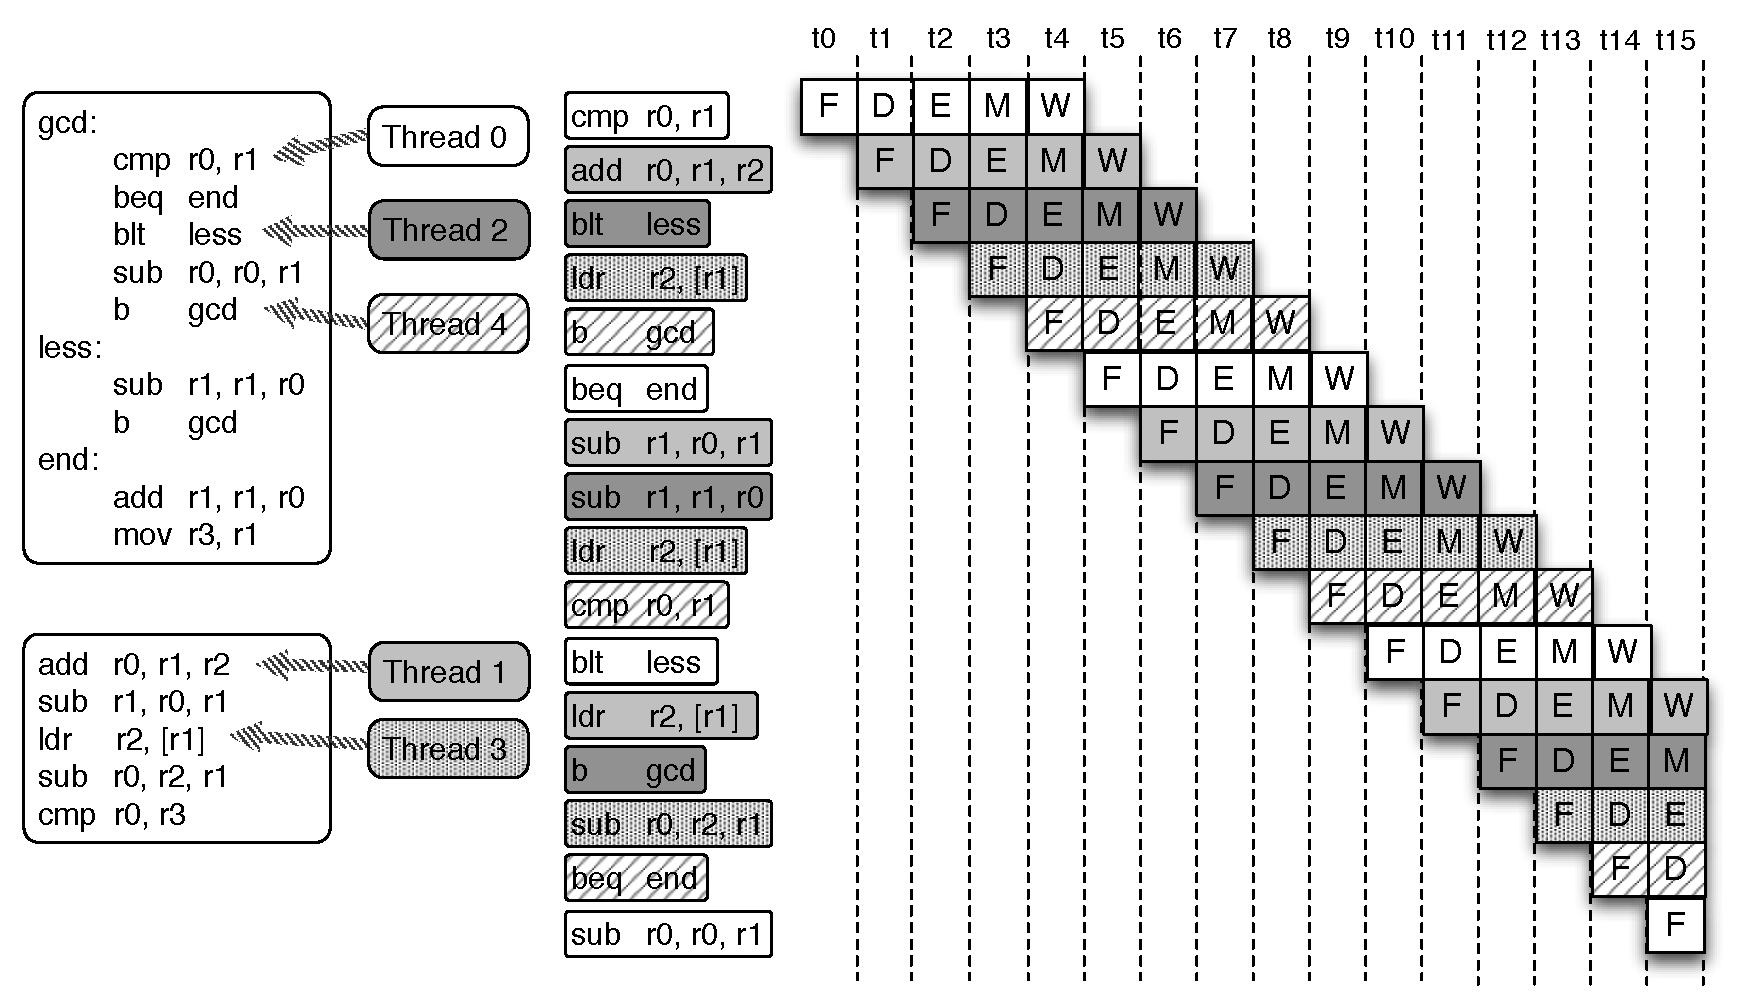
\includegraphics[scale=.55]{figs/thread-interleaved-execution}
  \end{center}
  \vspace{-10pt}
  \caption{Sample execution sequence of a thread-interleaved pipeline with 5 threads and 5 pipeline stages}
  \label{fig:execution_thread_interleaved_pipeline}
\end{figure}

The same code segments from figure~\ref{fig:sample_gcd_code} and figure~\ref{fig:sample_data_dependent_code} are used in this example. 
Threads 0, 2 and 4 execute GCD (figure~\ref{fig:sample_gcd_code}) and threads 1 and 3 execute the data dependent code segment (figure~\ref{fig:sample_data_dependent_code}).
The thick arrows on the left show the initial execution progress of each thread at cycle 0.
We observe from the figure that each cycle, an instruction from a different hardware thread is fetched in round robin order.
By cycle 4, each pipeline stage is occupied by a different hardware thread.
The fine-grained thread interleaving and round robin scheduling combine to form this important property for thread-interleaved pipelines, which provides the basis for a timing predictable pipeline design.

The interleaving of threads by itself does not guarantee timing predictability for the pipeline.  
Shared hardware components or a selective thread execution policy can easily allow the execution time of threads to be affected by each other.    
As previously discussed, a combined timing analysis of all threads in the pipeline is extremely difficult, if not impossible.
In order for multithreaded architectures to achieve predictable performance, threads must be temporally isolated from one another. 
Temporal isolation removes cross-thread timing dependencies to allow timing analysis of threads independently.
This enables a simple and more precise execution time analysis.  
We refine several features on the thread-interleaved pipeline to temporally isolate the threads and predictably handle pipeline hazards.
This establishes a time-predictable thread-interleaved pipeline.

\subsubsection{Control Hazards}
By interleaving enough threads, control hazards can be completely removed in thread-interleaved pipelines.
This can be observed from the execution sequence shown in figure~\ref{fig:execution_thread_interleaved_pipeline}.

At cycle 2, a \emph{blt} instruction from thread 2 is fetched into the pipeline.
In a single-threaded pipeline, a stall or branch prediction would be required before the next instruction fetch.
However, as the figure illustrates, the next instruction fetched (\emph{ldr}) at cycle 3 belongs to a different thread.
There is no control hazard in this case, because the \emph{ldr} instruction does not rely on the branch results of the \emph{blt} instruction.  
Thus, no stall or branch prediction is needed to fetch this instruction.
In fact, the branch result from \emph{blt} is not needed until cycle 7, when thread 2 is fetched again.
By this point, the branch has already been resolved, so no control hazard is caused from the \emph{blt} instruction.
The next fetched instruction from thread 2 is \emph{always} from the correct program path.
In this way, the control hazards from branches are eliminated.  
  
The interleaving of threads also eliminates control hazards in the presence of exceptions.
If the pipeline detects an exception for the \emph{blt} instruction in its writeback stage (cycle 6), the control flow for thread 2 will be changed to handle the exception.  
Because no other instruction in the pipeline belongs to thread 2 at cycle 6, no instruction needs to be flushed.  
This reveals an important property our timing predictable pipeline, that \emph{no instruction is speculatively executed}.
The next instruction fetch from thread 2 does not occur until cycle 7.
At that point, any control flow change, including one caused by an exception, is already known.
Therefore, the correct program path is always executed.

The minimum number of threads required to eliminate control hazards depends on the number of the pipeline stages.
Conservatively, interleaving the same number of threads as pipeline stages will always remove control hazards.
Intuitively, this is because at any point in time, each stage of the pipeline will be executing an instruction from a different hardware thread. 
Thus, no explicit dependency will exist between instructions in the pipeline. 
Lee and Messerschmitt~\cite{lee1987pip} further showed that it is possible to use one less thread than the number of pipeline stages for certain implementations. 
From here on, when we refer to the thread-interleaved pipeline, we assume enough threads to remove \emph{explicit} dependencies between instructions in the pipeline.
	
Because control hazards are eliminated, branch predictors are not needed in our pipeline design. 
Removing the branch predictor contributes to the temporal isolation of threads, as the shared internal state of the branch predictor can create \emph{implicit} dependencies between threads.  

\subsubsection{Data Hazards}
In a thread-interleaved pipeline, data hazards that stem from the pipelining of instructions are removed.  
The same reasoning for control hazard elimination is applied here, that no \emph{explicit} dependencies exist between instructions in the pipeline, 
However, long latency operations can still cause data hazards in a thread-interleaved pipeline. 
This happens when a long latency operation is not completed before the next instruction fetch from the same thread.
Although thread-interleaved pipelines can continue to fill the pipeline with other threads, if all threads simultaneously execute a long latency operation, then no thread will be available to fill the pipeline. 

To maximize pipeline utilization and instruction throughput, thread-interleaved pipelines can mark threads inactive for long latency operations.   
However, this dynamic thread scheduling leads to non-trivial timing effects for the pipeline. 
First, the number of active threads can fall below the minimum number of threads required to remove explicit dependencies of instructions in the pipeline.
In this case, the eliminated control and data hazards are now reintroduced, and hazard handling logic, like the branch predictor, is required again. 
%As a result, the timing effects of branch prediction etc are re-introduced in the pipeline. 
%By allowing threads to be inactive, it is possible for the number of active threads to fall below this minimum. 
This can be circumvented by inserting pipeline stalls when the number active threads falls below the minimum.
This is illustrated in figure~\ref{fig:three_thread_pipeline}.
\begin{figure}[h]
  \vspace{-10pt}
  \begin{center}
    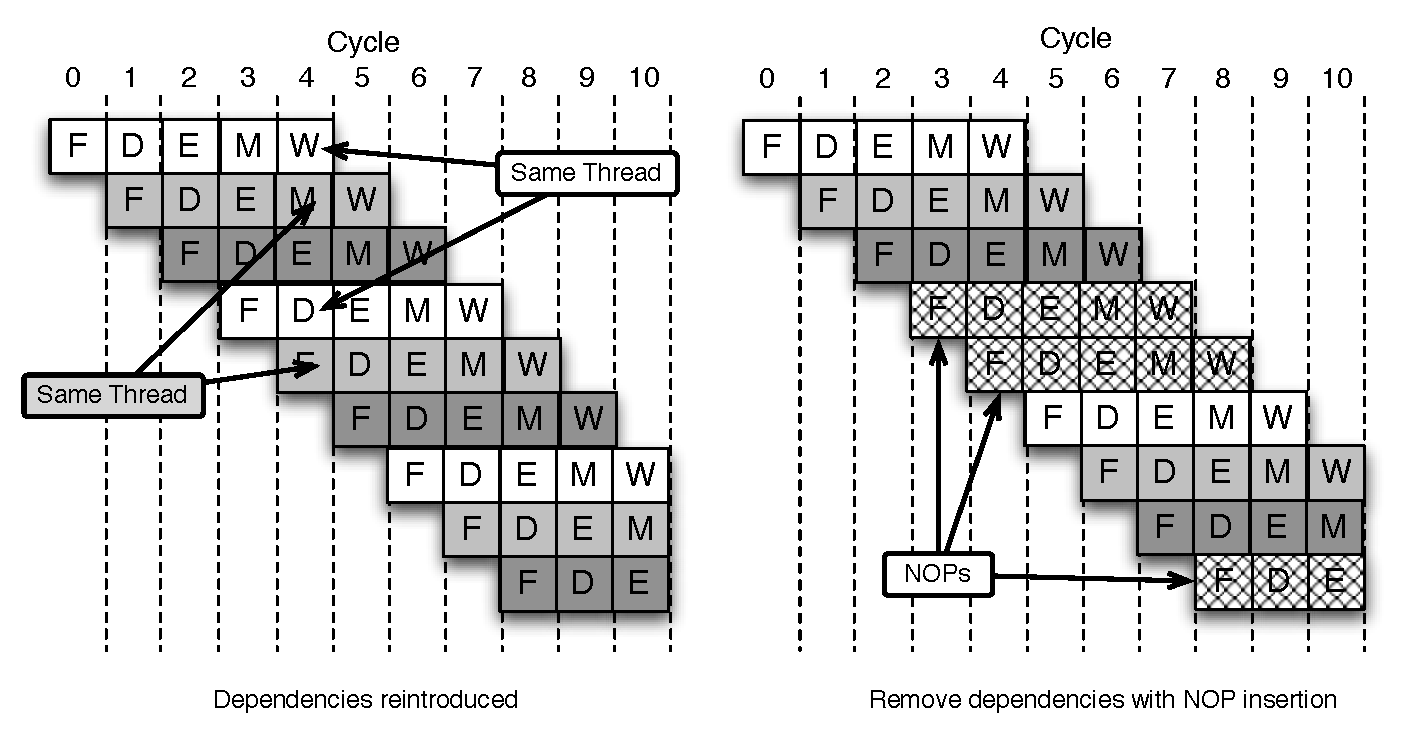
\includegraphics[scale=.6]{figs/three_thread_pipeline}
  \end{center}
  \vspace{-10pt}
  \caption{Execution of 5 threads thread-interleaved pipeline when 2 threads are inactive}
  \label{fig:three_thread_pipeline}
\end{figure}
In the figure, 3 (out of 5) threads are interleaved through a 5 stage pipeline. 
We assume that the other 2 threads are inactive waiting for memory access.    
On the left we show that explicit dependencies between instructions in the pipeline are reintroduced.
However, by inserting pipeline stalls to meet the minimum required thread count, the dependencies are once again removed.
This is shown on the right.   
Employing more total threads in the pipeline can reduce the amount of stalling needed, since there is a larger pool of threads to select from.  
However, to ensure that explicit dependencies are removed, stalls are \emph{always} required when the active thread count drops below the minimum.

More importantly however, the dynamic activation and deactivation of threads breaks temporal isolation between the threads.   
When a thread is deactivated, other threads are fetched more frequently into the pipeline.
At any one moment, the execution frequency of threads would depend on the number of active threads. 
Because a thread can deactivate based upon its own execution and affect other threads' execution frequency, threads are no longer temporally isolated.

In order to maintain temporal isolation between the threads, threads cannot affect the execution time of others.
For a time-predictable thread-interleaved pipeline, threads are not dynamically deactivated.
Instead, when a thread is fetched in the presence of a data hazard, a pipeline delay is inserted to preserve the round robin thread schedule.
This only slightly reduces the utilization of the pipeline, as other threads are still executing during the long latency operation.
But the temporal isolation of threads is preserved, as the execution frequency of threads remains the same regardless of any thread activity.  
Compared to single threaded pipelines, the benefits of latency hiding from mulithreading are still present.

%The next instruction from thread 3 that is fetched into the pipeline is again the same \emph{ld} instruction.  
%As memory completes its execution during the execution of instructions from other threads, we replay the same instruction to pick up the results from memory and write it into registers to complete the execution of the \emph{ld} instruction. 
%It is possible to directly write the results back into the register file when the memory operation completes, without cycling the same instruction to pick up the results.
%This would require hardware additions to support and manage multiple write-back paths in the pipeline, and a multi write ported register file, so contention can be avoided with the existing executing threads.
%In our design we simply replay the instruction for write-backs to simplify design and piggy back on the existing write-back datapath.

Because no \emph{explicit} dependency exists between the instructions in the pipeline, the forwarding logic used to handle data hazards can be stripped out in thread interleaved pipelines. 
Data forwarding logic contains no internal state, so threads are temporally isolated even if it is present.   
However, the pipeline datapath can be greatly simplified in the absence of forwarding logic and branch predictors.
The static thread schedule reduces the overhead of context switches to almost none; it can be implemented with a simple $log(n)$ bit up-counter, where $n$ is the number of threads.     
This enables thread-interleaved pipelines to be clocked at faster clock speeds, because less logic exists between each pipeline stage.
  
\subsubsection{Structural Hazards}
Threads on a multithreaded architecture, by definition, share the underlying pipeline datapath and any hardware unit implemented in it.
Thus, multithreaded architectures are more susceptible to structural hazards, which can break temporal isolation if not handled predictably.

In multithreaded pipelines with a width of one, shared single-cycle hardware units do not cause structural hazards, because no contention arises from the pipelined instruction access.
However, multi-cycle hardware units cause structural hazards when consecutive instructions access the same unit. 
The second instruction needs to wait for the first to complete before obtaining access.
For thread-interleaved pipelines, this causes timing interference between threads, because consecutive instruction fetches come from different threads.
One thread's access to a multi-cycle hardware unit can cause another to delay.

If it is possible to pipeline the multi-cycle hardware unit to be single-cycle accessible, the structural hazard and timing interference can be eliminated.   
In our time-predictable thread interleaved pipeline, floating point hardware units are pipelined to be single-cycle accessible. 
Hence, they are shared predictably between the hardware threads, and cause no timing interference. 

If pipelining is not possible, then the management of contention for the hardware unit becomes essential to achieve temporal isolation of threads.     
The single memory unit in a thread-interleaved pipeline is an example of a shared, multi-cycle, non-pipeline-able hardware unit.
In this situation, a time division multiplex access (TDMA) schedule can be enforced to remove timing interference.
The TDMA schedule divides the access channel to the hardware unit into multiple time slots.  
Each thread only has access to the hardware unit at its assigned time slots, even if no other thread is currently accessing the unit.
By doing so, the access latency to the hardware unit is determined only by the timing offset between the thread and its access slot, not the activities of the other threads.
In section~\ref{section:memory_system} we show a predictable DRAM memory controller that use TDMA in the backend to schedule accesses to DRAM memory. 

It is important to understand that a TDMA schedule removes timing interference, but does \emph{not} remove structural hazards.
In fact, a TDMA schedule can further expose the performance penalty of structural hazards.
By reserving privatized time slots for threads, the hardware unit will appear to be busy even when no thread is accessing it.
Thus, structural hazards can occur even when the hardware unit is not being used.
Although a TDMA schedule increases the average latency to access the hardware unit, the worst-case access latency is similar that of a conventional first-come-first-serve (FCFS) queuing based access schedule with a queue size of one.
In both cases, the worst-case access latency needs to account for the accesses of all threads.      
However, by using a TDMA schedule to predictably handle the structural hazards, the temporal isolation of threads enable a much tighter and simpler WCET analysis~\cite{Lv:2010:CAI:1935940.1936246}.
%http://user.it.uu.se/~yi/pdf-files/RTSS10_65.pdf

% However, because the TDMA access schedule is static, and access time is decoupled from other threads, there is potential to obtain tighter timing analysis for accesses by inferring access slot hits and misses for future accesses. 
% For example, based upon the execution time offsets of a sequence of accesses to the shared resource, we may be able to conclude that at least one access will hit its TDMA access slot and get access right away.
% We can also possibly derive more accurate wait times for the accesses that do not hit its access slots based upon the elapsed time between accesses.
% An in depth study of WCET analysis of TDMA access schedules is beyond the scope of the thesis.
%But these are possibilities now because there is no timing interference between the threads. 
%A queue based mechanism would not be able to achieve better execution time analysis without taking into account the execution context of all other threads in the pipeline.

Even though shared single-cycle hardware units do not cause structural hazards, they can still introduce timing interference between threads in multithreaded architectures. 
Shared hardware units can create \emph{implicit} dependencies between threads if the internal hardware states can be updated by any thread. 
A shared branch predictor, as discussed earlier, is a prime example for this. 
Our thread-interleaved pipeline removes the need for a branch predictor by the interleaving of hardware threads.  
A shared cache is another example.   
A cache maintains internal state that determines whether a memory access goes to the cache or to the main memory.
There is typically an enormous latency difference between the two different accesses.
When the cache is shared between threads, the different interleaving of threads can affect the execution time of all threads. 
It is even possible to degrade the performance of the system if threads continuously evict cache lines from each other. 
This phenomenon is known as \emph{cache thrashing}.
Partitioned caches~\cite{cachepartition} in this case can be used to enforce separate internal states, so each thread updates only its own internal state.  
Our time-predictable thread-interleaved pipeline employs scratchpads instead of caches.
We discuss this in the context of a timing predictable memory hierarchy in section~\ref{section:memory_system}.   

As a side note, the sharing of internal hardware states between threads also increases security risks in multithreaded architectures. 
Side-channel attacks on encryption algorithms~\cite{Kelsey98sidechannel} exploit the shared hardware states to disrupt and probe the execution time of threads running the encryption algorithm.
The timing information can be used to crack the encryption key.
We show in section~\ref{sec:app_side_channel_attack} how our predictable thread-interleaved pipeline prevents timing side-channel attacks for encryption algorithms.   

\subsubsection{Deterministic Execution}
The time-predictable thread-interleaved pipeline uses multithreading to improve instruction throughput, and maintains temporal isolation of threads to achieve deterministic execution.  
To highlight these features, we show the isolated execution of threads within a thread-interleaved pipeline.
We use the example shown earlier (in figure~\ref{fig:execution_thread_interleaved_pipeline}), where we execute the sample GCD (figure ~\ref{fig:sample_gcd_code}) and data-dependent (figure ~\ref{fig:sample_data_dependent_code}) code on a 5 thread 5 stage thread-interleaved pipeline.   
Figure~\ref{fig:thread_isolated_execution} shows the execution of the first two threads in isolation. 
Thread 0 executes GCD, and thread 1 executes the data-dependent code.

\begin{figure}[h]
\begin{center}
\noindent\makebox[\textwidth]{%
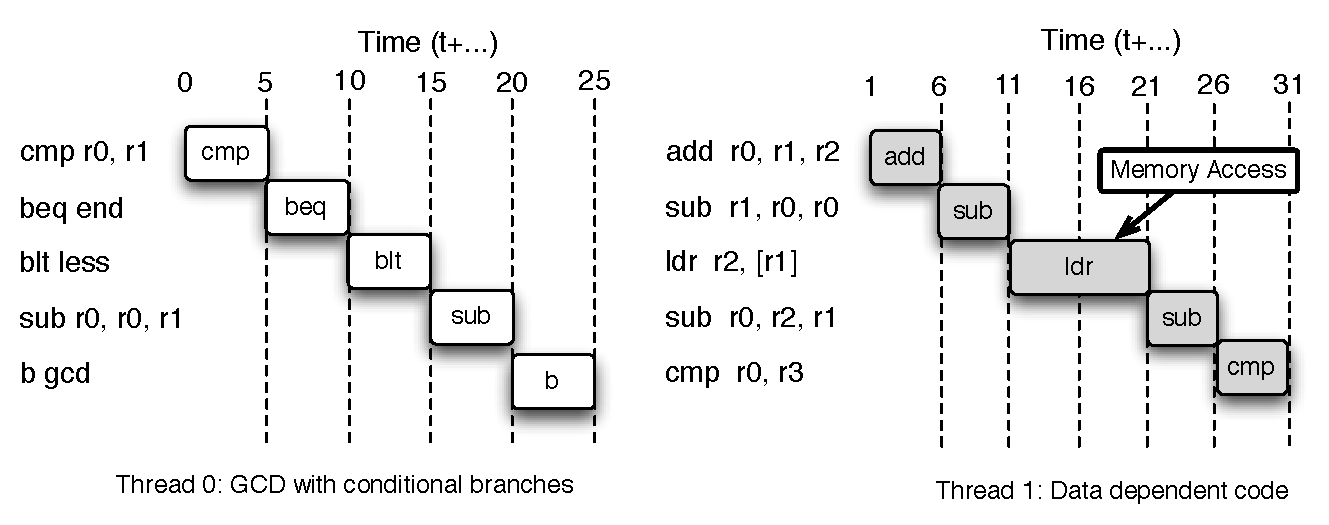
\includegraphics[scale=.58]{figs/thread_isolated_execution}}
\end{center}
\vspace{-3mm}
\caption{Isolated execution of threads with a thread-interleaved pipeline}
\label{fig:thread_isolated_execution}
\end{figure}

From the perspective of a thread, most instructions observe a 5 cycle latency, as shown in figure~\ref{fig:thread_isolated_execution}. 
The minimum observable latency for instructions depend on the number of threads executing in the pipeline. 
This can also be understood as the latency for each thread between instruction fetches.
In our time-predictable thread-interleaved pipeline, the static round robin thread schedule enables this latency to be constant.  
We use the term \emph{thread cycle} to encapsulate this latency, and simplify the numbers for timing analysis. 
In our example, the instructions shown in thread 0 each take 1 thread cycle.

The \emph{ldr} instruction in thread 1 accesses main memory.
From the thread-interleaving, the access latency to main memory is hidden in the concurrent execution of other threads. 
Thus, long latency instructions can appear to have a reduced latency in the isolated view of threads.
In this example, the \emph{ldr} instruction observes only a 2 thread cycle latency, even though the actual memory access latency could have been up to 10 processor cycles. 

Threads are temporally isolated in our thread-interleaved pipeline, so execution of each thread can be analyzed in isolation.
From the isolated view of each thread, each instruction completes its execution before the next one is fetched, and no instruction is executed speculatively.
Because instructions do not overlap in execution, each instruction's execution time is not affected by prior instructions.
Control hazards are eliminated because a branch or exception is resolved before the next instruction fetch. 
The long latencies caused by structural or data hazards are hidden from the thread interleaving, improving the throughput of the pipeline.    
We will describe in detail our implementation of the thread-interleaved pipeline in the beginning of chapter ~\ref{chapter:ptarm}.

\section{Memory System}
\label{section:memory_system}
While pipelines designs continue to improve, memory technology has been struggling to keep up with the increase in clock speed and performance.
Even though memory bandwidth can be improved with more bank parallelization, the memory latency remains the bottleneck to improved memory performance.
Common memory technologies used in embedded systems contain a significant tradeoff between access latency and capacity. 
Static Random-Access Memories (SRAM) provide a shorter latency that allows single cycle memory access from the pipeline.
However, the hardware cost to implement each memory cell prevents SRAM blocks from being implemented with high capacity.
On the other hand, Dynamic Random-Access Memories (DRAM) use a more compact memory cell design that can easily be combined into larger capacity memory blocks.
But the memory cell of DRAMs must be constantly refreshed due to charge leakage, and the large capacity memory blocks often prohibit faster access latencies.
%TODO: talk about about embedded systems seldom need disk?
To bridge the latency gap between the pipeline and memory, smaller memories are placed in between the pipeline and larger memories to act as a buffer, forming a memory hierarchy.
The smaller memories give faster access latencies at the cost of lower capacity, while larger memories make up for that with larger capacity but slower access latencies. 
The goal is to speed up program performance by placing commonly accessed values closer to the pipeline and placing less accessed values farther away.

\subsection{Memory Hierarchy}
\subsubsection{Caches}
\begin{wrapfigure}{r}{0.5\textwidth}
  \vspace{-20pt}
  \begin{center}
    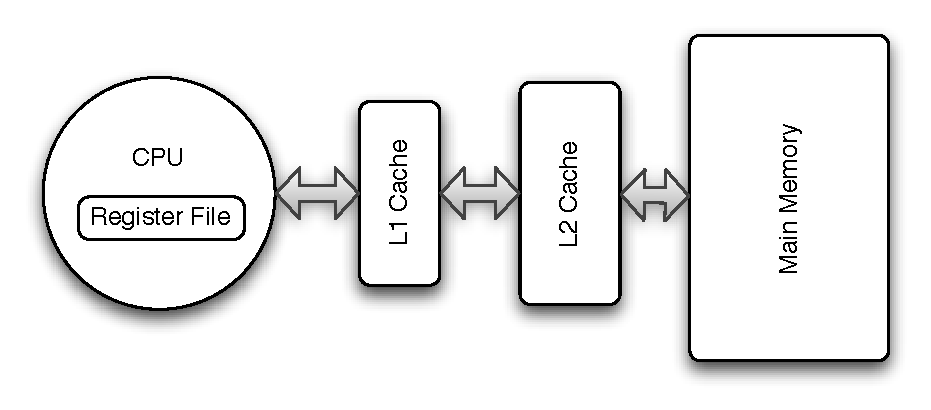
\includegraphics[scale=.5]{figs/conventional_mem_hierarchy}
  \end{center}
  \vspace{-20pt}
  \caption{Memory Hierarchy w/ Caches}
  \label{fig:conventional_mem_hierarchy}
  \vspace{-10pt}
\end{wrapfigure}   
A \emph{CPU Cache} (or cache) is commonly used in the memory hierarchy to manage the smaller fast access memory made of SRAMs.
The cache manages the contents of the fast access memory in hardware by leveraging the spatial and temporal locality of data accesses. 
The main benefits of the cache is that it abstracts away the memory hierarchy from the programmer.
When a cache is used, all memory accesses are routed through the cache. 
If the data from the memory access is in the cache, then a cache hit occurs, and the data is returned right away.
However, if data is not in the cache, then a cache miss occurs, and the cache controller fetches the data from the larger memory and adjusts the memory contents in the cache. 
The replacement policy of the cache is used to determine which cache line, the unit of memory replacement on caches, to replace. 
A variety of cache replacement policies have been researched and used to optimize for different memory access patterns of applications. 
In fact, modern memory hierarchies often contain multiple layers of hierarchy to balance the tradeoff between speed and capacity.
A commonly used memory hierarchy is shown in figure~\ref{fig:conventional_mem_hierarchy}.
If the data value is not found in the L1 cache, then it is searched for in the L2 cache. 
If the L2 cache also misses, then the data is retrieved from main memory, and sent back to the CPU while the L1 and L2 cache update its contents.
Different replacement policies can be used at different levels of the memory hierarchy to optimize the hit rate or miss latency of the memory access.

When caches are used, the program is oblivious to the different levels of memory hierarchy because they are abstracted away from the program; the cache gives its best-effort to optimize memory access latencies.
Whether or not an access hits the cache or goes all the way out to main memory is hidden from the program.
Thus, the programmer does not need to put in any effort, and can get a reasonable amount of performance. 
Furthermore, when programs are ported to another architecture with a different cache configuration, no change in the program is required to still obtain a reasonable amount of performance from the hardware.   
For general purpose applications, this gives the ability to improve design time and decrease design effort, which explains the cache's popularity. 

However, the cache makes no guarantees on actual memory access latencies and program performance. 
The execution time of programs could highly vary depending on a number different factors -- cold starts, previous execution contexts, interrupt routines, and even branch mispredictions that cause unnecessary cache line replacements.  
Thus, when execution time is important, the variability and uncontrollability of caches may outweigh the benefits they provide. 

The cache's internal states include the controller state and memory contents. 
As the programmer cannot explicitly control the state of the cache, it is extremely difficult to analyze execution time on systems with caches.
At an arbitrary point of execution, if the state of the cache is unknown, a conservative worst-case execution time analysis needs to assume the worst case, as if the memory access went directly to main memory.
In order to acquire tighter execution time analysis, the cache must be modeled with program execution to predict the cache state.
The ease of such modeling depends on the replacement policy used in the cache.

For example, the \emph{Least Recent Used} (LRU) replacement policy replaces the least recently used cache line whenever an eviction occurs. 
Within a basic block, a code segment without a control flow change, the contents of a cache with $N$ cache lines can be fully known after $N$ different memory accesses~\cite{Heckmann2003processor}.  
The $N$ different memory accesses will evict all cache lines in the cache prior to the basic block, and fill them with the memory contents of the $N$ accesses. 
In this case, the analysis assumes $N$ initial cache misses before the cache state is known.
However, the cache state is destroyed when analysis hits a control flow merge with another path.
Thus, the usefulness of this analysis depends on $N$ and how long basic blocks are in programs.  
In practice, the complexity of modern programs and memory architectures often introduce a high variability in program execution time, rendering analysis imprecise. 

Even outside of the context of real-time applications, caches can present unintended side effects.
For applications that require extreme high speed, the best-effort memory management that caches offer simply is not good enough.
Programs often need to be tuned and tailored to specific cache architectures and parameters to achieve the desired performance. 
In order to tune algorithm performance, algorithm designers are required to understand the abstracted away memory architecture and enforce data access patterns that conform to the cache size and replacement policy.   
For example, instead of operating on entire rows or columns of an array, algorithms are rewritten to operate on a subset of the data at a time, or blocks, so the faster memory in the hierarchy can be reused.
This technique is called \emph{Blocking}~\cite{Lam91thecache}, and is very well-known and commonly used.   
%\todo{talk about LAPACK? Libraries that tune programs to caching}.
%In this case, we see that the hidden memory hierarchy actually could degrade program performance.    

Multithreaded threaded architectures with shared caches among the hardware threads can suffer from \emph{cache thrashing}, an effect where different threads' memory accesses evict the cached lines of others.
With multiple hardware threads, it is extremely difficult for threads have any knowledge on the state of the cache, because it is simultaneously being modified by other threads in the system. 
As a result, the hardware threads have no control over which level in the memory hierarchy they are accessing, and the performance highly varies depending on what is running on other hardware threads. 

For multicore architectures, caches create a data coherency problem when data needs to be consistent between the multiple cores.
When the multiple cores are sharing memory, each core's private cache may cache the same memory address. 
If one core writes to a memory location that is cached in its private cache, then the other core's cache would contain stale data. 
Various methods such as bus snooping or implementing a directory protocol~\cite{Stenstrom:1990:SCC:79809.79810} have been proposed to keep the data consistent in all caches. 
Implementing a scalable and efficient cache coherence scheme is still a hot topic of research today.

\subsubsection{Scratchpads}
We cannot argue against the need for a memory hierarchy, as there is an undeniable gap between processor and DRAM latency.
However, instead of abstracting away the memory hierarchy, we propose to \emph{expose} the memory layout to the software.  

\emph{Scratchpads} were initially proposed for their power saving benefits over caches~\cite{Banakar2002}.
Scratchpads can be found in the Cell processor~\cite{cellproc}, which is used in Sony PlayStation 3 consoles, and NVIDIA's 8800 GPU, which provides 16KB of SPM per thread-bundle~\cite{8800gpu}.
Scratchpads use the same memory technology (SRAMs) as caches, but do not implement the hardware controller to manage their memory contents.
%Without the hardware controller, scratchpads do not manage its memory contents in hardware.
Instead, scratchpads occupy a distinct address space in memory when they are used as fast access memory.
Memory accesses that access the specific scratchpad address space will go to the scratchpad, and other accesses will go to main memory. 
Because in hardware scratchpads do not need to check whether the data is on the scratchpad or not, they have a reduced access latency, area and power consumption compared to caches~\cite{Banakar2002}. 

\begin{wrapfigure}{r}{0.45\textwidth}
  \vspace{-20pt}
  \begin{center}
    \includegraphics[scale=.5]{figs/pret_mem_hierarchy}
  \end{center}
  \vspace{-10pt}
  \caption{Memory Hierarchy w/ Scratchpads}
  \label{fig:pret_mem_hierarchy}
\end{wrapfigure}   

Unlike caches, which overlay their address space with main memory to hide the hierarchy, scratchpads explicitly \emph{expose} the memory hierarchy, as figure~\ref{fig:pret_mem_hierarchy} illustrates.  
The exposed memory hierarchy gives software full control over the management of memory contents in the hierarchy.
Data allocated on the scratchpad will have single cycle access latencies, while other data will take the full DRAM access latency. 
The memory access latency for each request now depends only on the access address, and not that state of another hardware controller. 
This drastically improves the predictability of memory access times, and removes the variability of execution time introduced with caches.
However, this places the burden of memory management on the programmer or compiler toolchains.  
The Cell processor~\cite{cellproc} is often criticized for being difficult to program, and one of the main reason is its use of scratchpads. 
Programmers have become accustomed to a uniform memory space, making it difficult to adjust to the non uniform memory space that must be explicitly managed.

Embedded system designs inherently need to deal with limited resources and other design constraints, such as limited memory or hard timing deadlines.    
Thus, the design of such systems often requires analysis of memory usage and latency to ensure that the constraints are met.
These analysis results can be used to generate automatic allocation schemes for scratchpads, lessening the burden on programmers.
Two allocation schemes are commonly employed to manage the contents of scratchpads in software.
\emph{Static allocation schemes} allocate data on the scratchpad during compile time, and the contents allocated on the scratchpad do not change throughout program execution. 
Static scratchpad allocation schemes~\cite{Suhendra2005WCETSPM, Patel2008PRETSPM} often use heuristics or a compiler-based static analysis of the program to find the most commonly executed instructions or data structures.
These are allocated statically on the scratchpad to improve program performance. 
\emph{Dynamic allocation schemes} modify the data on the scratchpad during run time in software through DMA mechanisms.
The allocation could either be automatically generated and inserted by the compiler, or explicitly specified by the user programmatically.
Higher level models of computation, such as Synchronous Dataflow (SDF)~\cite{lee_sdf} or Giotto~\cite{henzinger_giotto}, expose more structure and semantics of the model for better analysis, which can be used to optimize scratchpad allocation dynamically.
Bandyopadhyay~\cite{Bandyopadhyay06_AutomatedMemoryAllocationOfActorCodeDataBufferInHeterochronous} presents an automated memory allocation of scratchpads for the execution of Heterochronous Dataflow models.
The Heterochronous Dataflow (HDF) model is an extension to the Synchronous Dataflow (SDF) model with finite state machines (FCM). 
The HDF models contain different program states.
Each state executes a SDF model that contains actors communicating with each other. 
Bandyopadhyay analyzes the actor code and the data that is communicated in each HDF state, and derives an optimized scratchpad allocation for each state. 
The scratchpad allocation code is automatically inserted into the code to dynamically change the scratchpad contents during state transitions, so the memory allocation is optimized for the execution of each HDF state. 
This allocation not only shows roughly a 17\% performance improvement compared to executions using LRU caches, but also a more predictable program performance.

The underlying memory technology that is used to make both scratchpads and caches is not inherently unpredictable, as SRAMs provide constant low-latency access time. 
%However, caches manage the contents of the SRAM in hardware. 
However, by using caches in the memory hierarchy, the hierarchy is hidden from the programmer, and the hardware managed memory contents create highly variable execution times with unpredictable access latencies. 
Scratchpads on the other hand expose the memory hierarchy to the programmer, allowing for more predictable and repeatable memory access performances.
Although the allocation of scratchpads requires more programming effort, it also provides opportunity for high efficiency, as it can be tailored to specific applications.   
Thus, in our time-predictable architecture, scratchpads are employed as our fast-access memory. 

\subsection{DRAM Memory Controller}
Because of its high capacity, DRAMs are often employed in modern embedded systems to cope with the increasing code and data sizes.  
However, bank conflicts and refreshes within the DRAM can cause memory accesses to stall, further increasing the memory latency. 
Modern memory controllers are designed to optimize average-case performance by queueing and reordering memory requests to improve the throughput of memory requests. 
This results in unpredictable and varying access times along with an increased worst-case access time for each memory request.
In this section we will present a DRAM memory controller that privatizes DRAM banks with scheduled memory refreshes to provide improved worst-case latency and predictable access times.    
The contributions from this section are research done jointly with the several co-authors from Reineke et. al~\cite{ReinekeLiuPatelKimLee11_PRETDRAMControllerBankPrivatizationForPredictability}. 
We do not claim sole credit for this work, and the summary is included in this thesis only for completeness. 
We will first give some basic background on DRAM memories, then present the predictable DRAM controller designed.

\subsubsection{DRAM Basics}

\begin{figure}[h]
\begin{center}
\vspace{-8mm}
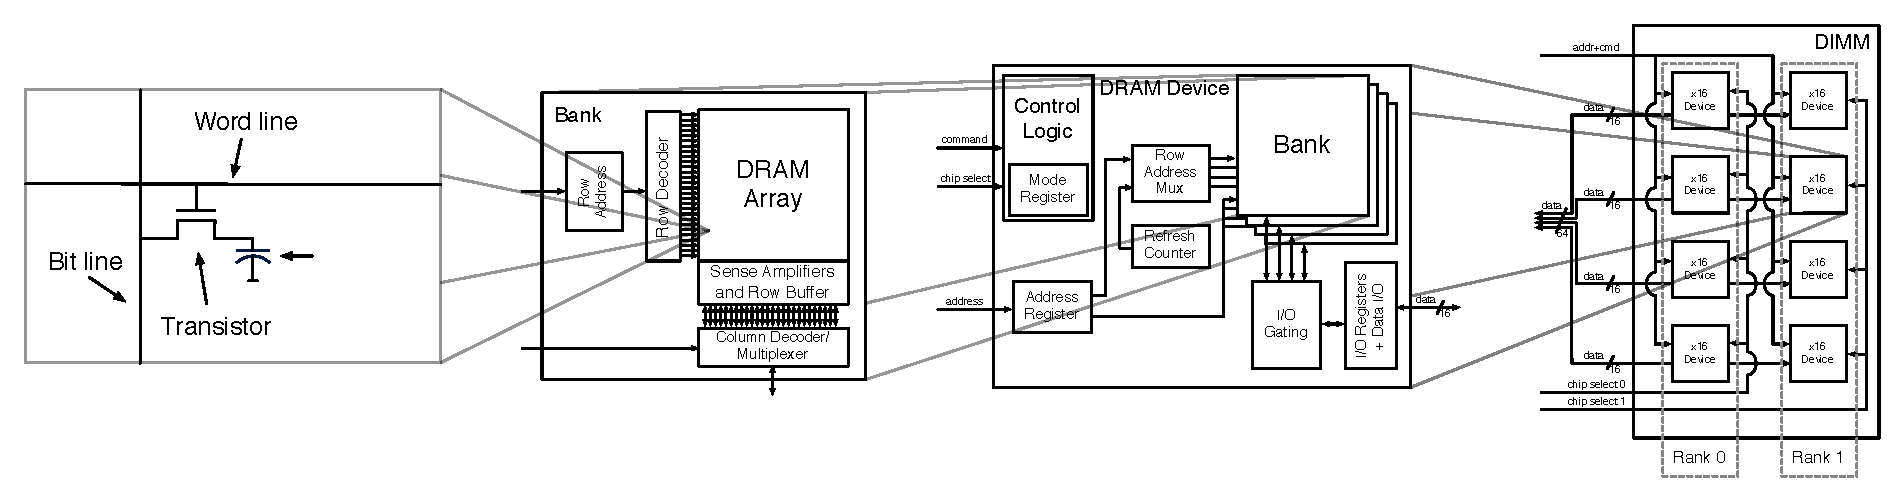
\includegraphics[width=\textwidth]{figs/dram-overview.pdf}
\vspace{-8mm}
\caption{A dual-ranked dual in-line memory module.}\label{fig:dram_basics}
\vspace{-5mm}
\end{center}
\end{figure} 

Figure~\ref{fig:dram_basics} shows the structure of a dual ranked in-line DDRII DRAM module.
Starting from the left, a basic \textbf{\emph{DRAM cell}} consists of a capacitor and a transistor. 
The capacitor charge determines the value of the bit, which can be accessed by triggering the transistor. 
Because the capacitor leaks charge, it must be refreshed periodically, typically every 64 ms or less~\cite{jedec}.

A \textbf{\emph{DRAM array}} is made of a two-dimensional array of DRAM cells.
Each access made to the DRAM array goes through two phases: a row access followed by one or more column accesses.   
During the row access, one of the rows in the DRAM array is moved into the row buffer.
To read the value in the row buffer, the capacitance of the DRAM cells is compared to the wires connecting them with the row buffer.
The wires need to be precharged close to the voltage threshold so the sense amplifiers can detect the bit value.
Columns can be read and written to quickly after the row is in the row buffer. 

The \textbf{\emph{DRAM device}} consists of banks formed of DRAM arrays. 
Modern DRAM devices have multiple banks, control logic, and I/O mechanisms to read from and write to the data bus, as shown in the center of figure \ref{fig:dram_basics}.
Banks can be accessed concurrently, but the data, command and address busses, which is what the memory controller uses to send commands to the DRAM device, are shared within the device. 
The following table\footnotemark\ lists the four most important commands and their function:
\footnotetext{This table is as shown in ~\cite{ReinekeLiuPatelKimLee11_PRETDRAMControllerBankPrivatizationForPredictability}}
%\begin{table}
\begin{center}
\begin{smalltabular}{p{13mm}p{6mm}p{10cm}}
Command 				& Abbr. & Description\\\hline
Precharge    			& PRE   & Stores back the contents of the row buffer into the DRAM array, and prepares the sense amplifiers for the next row access.\\
Row\hspace{13mm} access & RAS	& Moves a row from the DRAM array through the sense amplifiers into the row buffer.\\
Column access 			& CAS   & Overwrites a column in the row buffer or reads a column from the row buffer.\\
Refresh					& REF	& Refreshes several\footnotemark\ rows of the DRAM array. This uses the internal refresh counter to determine which rows to refresh.\\
\end{smalltabular}
%\caption{Overview of DDR2 Commands~\cite{ReinekeLiuPatelKimLee11_PRETDRAMControllerBankPrivatizationForPredictability}}
\label{tab:ddr2-commands}
\end{center}
%\end{table}
\footnotetext{The number of rows depends on the capacity of the device.}

To perform reads or writes, the controller first sends the PRE command to precharge the bank containing the data. 
Then, a RAS is issued to select the row, and one or more CAS commands can be used to access the columns within the row. 
Accessing columns from the same row does not require additional PRE and RAS commands, thus higher throughput can be achieved by performing column accesses in burst lengths of four to eight words.  
Column accesses can immediately be followed by a PRE command to decrease latency when accessing different rows. 
This is known as auto-precharge (or closed-page policy).
Refreshing of the cells can be done in two ways.
One common way is to issue a refresh command that refreshes all banks of the device simultaneously. 
The refresh latency depends on the capacity of the device, but the DRAM device manages a counter to step through all the rows.
The rows on the device could also be manually refreshed by performing row accesses to them.
Thus, the memory controller could perform row accesses on every row within the 64 ms refresh period.
This requires the memory controller to keep track of the refresh status of the device and issue more refresh commands, but each refresh takes less time because it is only a row access. 

\textbf{\emph{DRAM modules}} are made of several DRAM devices integrated together for higher bandwidth and capacity. 
A high-level view of the dual-ranked dual in-line memory module (DIMM) is shown in the right side of figure~\ref{fig:dram_basics}.
The DIMM has eight DRAM devices that are organized in two ranks.
The two ranks share the address, command inputs, and the 64-bit data bus.
The chip select is used to determine which ranks are addressed.
All devices within a rank are accessed simultaneously when the rank is addressed, and the results are combined to form the request response.  
% Due to the sharing of I/O mechanisms within a device, consecutive accesses to the same rank are more constrained than consecutive accesses to different ranks, which only share the command and address as well as the data bus.
% We later exploit this subtle difference by restricting consecutive accesses to different ranks to achieve more predictable access latencies.  
% We explain this in more detail in \ref{sec:pret_dram_controller}. 

Our controller makes use of a feature from the DDR2 standard known as posted-CAS.  
Unlike DDR or other previous versions of DRAMs, DDR2 can delay the execution of CAS commands (posted-CAS) for a user-defined latency, known as the additive latency ($AL$). 
Posted-CAS can be used to resolve command bus contention by sending the posted-CAS earlier than the corresponding CAS needs to be executed.

Table~\ref{table:ddr2-constraints} gives an overview of timing parameters for a DDR2-400 memory module.
These timing constraints come from the internal structure of DRAM modules and DRAM cells.
For example, $t_{RCD}, t_{RP}$, and $t_{RFC}$ are from the structure of DRAM banks that are accessed through sense amplifiers that need to be precharged.
$t_{CL}, t_{WR}, t_{WTR}$, and $t_{WL}$ result from the structure of DRAM banks and DRAM devices.
The four-bank activation window constraint $t_{FAW}$ constrains rapid activation of multiple banks that would result in too high of a current draw.
The memory controller must conform to these timing constraints when sending commands to the DDR2 module.  
%The additive latency, $t_{AL}$, can be set by the user and determines how many cycles after a posted-CAS a CAS is executed.
Here we only give a quick overview of DRAMs, we refer more interested readers to Jacob et al.~\cite{JaNgWa07} for more details.

\begin{table}[h]
\begin{center}
\begin{smalltabular}{l p{2.0cm} p{10cm}}
Parameter	& Value \footnotemark & Description \\\hline
$t_{RCD}$			& 3						& \textbf{Row-to-Column delay}: time from row activation to first read or write to a column within that row.\\
$t_{CL}$			& 3						& \textbf{Column latency}: time between a column access command and the start of data being returned.\\
$t_{WL}$			& $t_{CL}-1=2$			& \textbf{Write latency}: time after write command until first data is available on the bus.\\
$t_{WR}$			& 3						& \textbf{Write recovery time}: time between the end of a write data burst and the start of a precharge command.\\
%$t_{CCD}$			& $\burstlength/2$ 				& CAS to CAS command delay. Minimum time between two read commands or two write commands.\\
$t_{WTR}$ 			& 2 					& \textbf{Write to read time}: time between the end of a write data burst and the start of a column-read command.\\% Allows the sense amplifiers to restore the data in the DRAM array.\\
$t_{RP}$			& 3						& \textbf{Row precharge time:} time to precharge the DRAM array before next row activation.  \\
%$t_{RTRS}$			& 1\todo{check this}	& Rank-to-rank switching time.\\ 
$t_{RFC}$			& 21					& \textbf{Refresh cycle time}: time interval between a refresh command and a row activation.\\
%$t_{REFI}$			& 1560    				& Refresh to refresh interval \\
%$t_{RAS}$ 			& $t_{RCD}+t_{WL}+t_{WR} = 8$ & Minimum time after an activate command to a bank until that bank is allowed to be precharged.\\
%$t_{RC}$			& $t_{RAS}+t_{RP}=11$	& Row cycle time: minimum time between successive activate commands to the same bank.\\
%$t_{RTP}$			&   			& Minimum time between a precharge command on a bank and a successive activate command.\\
$t_{FAW}$			& 10					& \textbf{Four-bank activation window}: interval in which maximally four banks may be activated.\\
$t_{AL}$			& set by user			& \textbf{Additive latency}: determines how long posted column accesses are delayed.
\end{smalltabular}
%\todo{group constraints by their origin: constraints due to DRAM array structure, constraints due to sharing within DRAM device, constraints due to sharing of bus among ranks}
\end{center}
\caption{Overview of DDR2-400 timing parameters of the Qimonda HYS64T64020EM-2.5-B2.~\cite{ReinekeLiuPatelKimLee11_PRETDRAMControllerBankPrivatizationForPredictability}}\label{table:ddr2-constraints}
\end{table}
\footnotetext{In cycles at 200 MHz}

\subsubsection{Predictable DRAM Controller}
\label{sec:pret_dram_controller}
We will split the discussion of the predictable DRAM controller into its backend and frontend. 
The backend translates memory requests into DRAM commands that are sent to the DRAM module.
The frontend manages the interface to the pipeline along with the responsibility of scheduling refreshes.
Here we specifically refer to a DDR2 667MHz/PC2-5300 memory module operating at 200Mhz, which has a total size of 512MB over two ranks with four banks on each rank.
While our discussion of the design of this DRAM controller is specific to our DDR2 memory module, the key design features are applicable to other modern memory modules.

\paragraph{Backend}
Conventional DRAM memory controllers view the entire memory device as one resource, and any memory request can access the whole DRAM device. 
Subsequent memory accesses can target the same bank within the DRAM, which results in the need for memory requests to be queued and serviced sequentially, without exploiting bank parallelism.
Our controller views the memory devices as independent resources partitioned by banks. 
Specifically, we partition our memory module into four \emph{resources}, each consisting of two banks within the same rank. 
The banks within each resource can be arbitrarily chosen, but all banks within a resource must belong to the same rank, and each of the ranks must contain at least two resources.
This is to avert access patterns that would incur high latency from the contention for the shared busses within banks and ranks.
The partitioning of the memory device allows us to fully exploit bank parallelism by accessing the resources in a periodic and pipelined fashion.
The periodic access scheme to the four resources interleaves each memory access between the ranks.
Subsequent accesses to the same rank go to the other resource, grouped from banks.  
Figure~\ref{fig:backend} shows an example of the following access requests: read from resource 0 in rank 0, write to resource 1 in rank 1, and read from resource 2 in rank 0. 

\begin{figure}[h]
\begin{center}
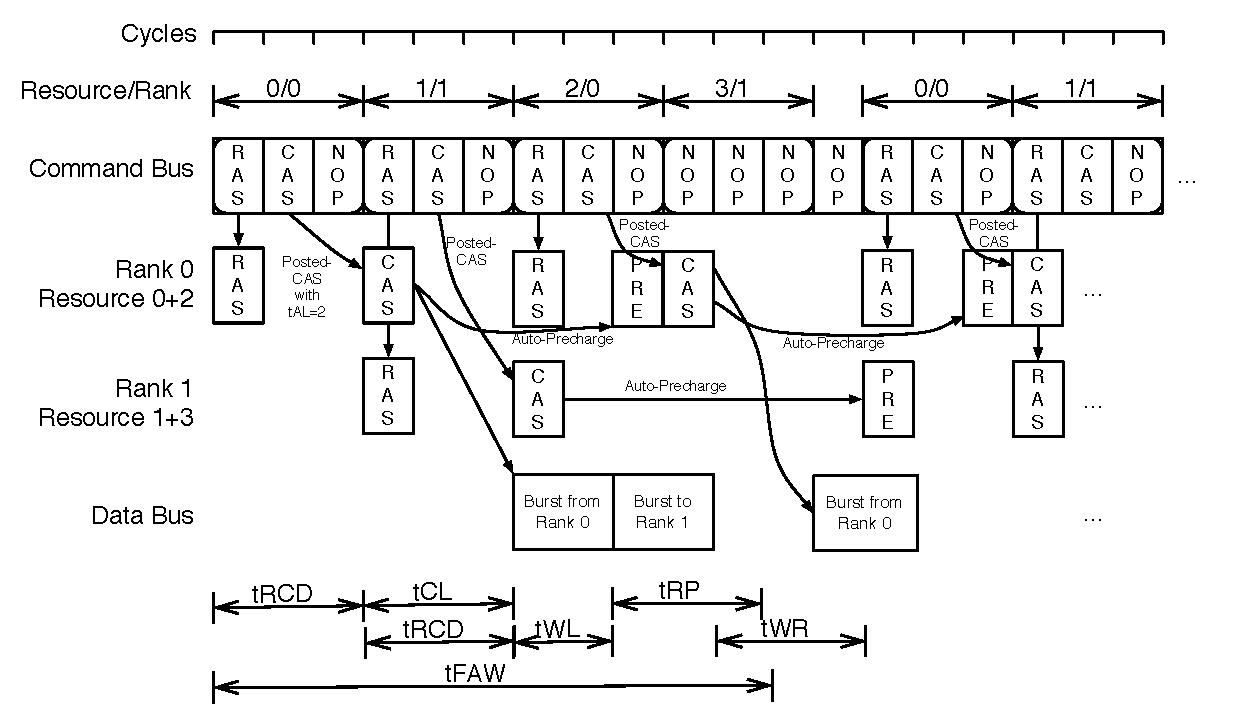
\includegraphics[width=0.92\linewidth]{figs/backend}
\end{center} 
\caption{The periodic and pipelined access scheme employed by the backend~\cite{ReinekeLiuPatelKimLee11_PRETDRAMControllerBankPrivatizationForPredictability}.}
\label{fig:backend}
\end{figure}

Each access request is translated into a RAS (Row Access), posted-CAS (Column Access) and NOP command. 
An access slot is formed of all three commands.  
The NOP command in the access slot is inserted between any two consecutive requests to avoid a collision on the data bus that occurs when a read request follows and a write request.
This collision is cause by the one cycle offset between the read and write latencies. 
The RAS command moves a row into the row buffer, and the CAS command accesses the columns within the row loaded into the row buffer. 
CAS commands can be either reads or writes, causing a burst transfer of $8 \cdot 4 = 32$ bytes that occupies the data bus for two cycles (as two transfers occur in every cycle).
We send a posted-CAS instead of a normal CAS in order to meet the row to column latency shown in table~\ref{table:ddr2-constraints}.
This latency specifies that the RAS command and the first CAS command need to be 3 cycles apart.  
However, manually issuing a CAS command to the first resource 3 cycles after its RAS command would cause a command bus conflict with the RAS command for the second resource.
Thus, we instead set the additive latency $t_{AL}$ to 2 and use the posted-CAS that offsets the CAS command to conform to the row to column latency.
This allows our memory controller to preserve our pipelined access scheme while meeting the latency requirements of the DRAM.   
We use a closed-page policy (also known as auto-precharge policy), which causes the accessed row to be immediately precharged after performing the column access (CAS), preparing it for the next row access.
If there are no requests for a resource, the backend does not send any commands to the memory module, as is the case for resource 3 in figure~\ref{fig:backend}.

Our memory design conforms to all the timing constraints listed in table~\ref{table:ddr2-constraints}.
The write-to-read timing constraint $t_{WTR}$, incurred by the sharing of I/O gating within ranks, is satisfied by alternating accesses between ranks. 
The four-bank activation window constraint is satisfied because within any window of size $t_{FAW}$ we activate at most four banks within the periodic access scheme. 
Write requests with the closed-page policy requires 13 cycles to access the row, perform a burst access, and precharge the bank to prepare for the next row access.
However, our periodic access scheme has a period of 12 cycles, as each access slot is 3 cycles, and there are four resources accessed. 
Thus, a NOP is inserted after the four access slots: to increase the distance between two access slots belonging to the same resource from 12 to 13 cycles.
As a result, the controller periodically provides access to the four resources every 13 cycles.
The backend does not issue any refresh commands to the memory module.
Instead, it relies on the frontend to refresh the DRAM cells using regular row accesses.

% \paragraph{Longer Bursts for Improved Bandwidth}
% Depending on the application, bandwidth might be more important than latency.
% Bandwidth can be improved by increasing the burst length from 4 to 8.
% Extending the proposed access scheme to a burst length of 8 is straightforward with the insertion of two additional NOP commands after each request to account for the extra two cycles of data being transfered on the data bus.  
% In this case, the access slot latency for each request is increased from three to five to include the extra two NOP commands, and data will be transferred in four out of five cycles rather than in two out of three.
% Then, of course, latency of transfers of size less than or equal to 32 bytes increases, but the latency of large transfers decreases and higher bandwidth is achieved. 

\begin{wrapfigure}{r}{0.5\textwidth}
\begin{center}
\vspace{-8mm}
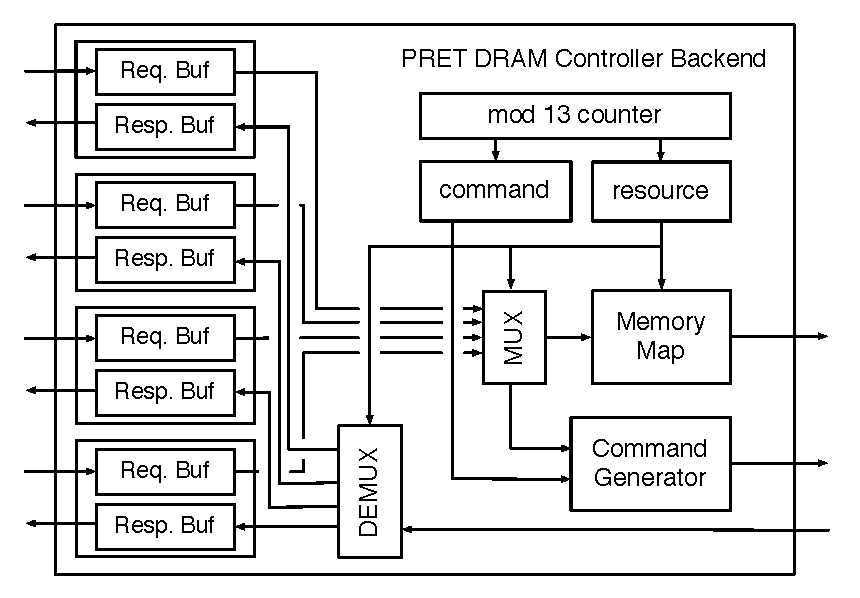
\includegraphics[width=1.1\linewidth]{figs/dram-backend-implementation}
\end{center}
\caption{Sketch of implementation of the backend~\cite{ReinekeLiuPatelKimLee11_PRETDRAMControllerBankPrivatizationForPredictability}.}
\label{fig:dram-backend-implementation}
\end{wrapfigure}

A high level block view of our backend implementation is shown in figure~\ref{fig:dram-backend-implementation}.
Each resource has a single request buffer and a respond buffer.
These buffers are used to interface with the frontend.   
A request is made of an access type (read or write), a logical address, and the data to be written for write requests. 
Requests are serviced at the granularity of bursts, i.e. 32 bytes in case of burst length 4 and 64 bytes in case of burst length 8.
A modulo-13 counter is used to implement the 13 cycle periodic access scheme in our controller.   
The ``resource'' and ``command" blocks are combinational circuits that are used to select the correct request buffer and generate the DRAM commands to be sent out. 
The ``memory map" block is where logical addresses are mapped to physical addresses that determine the rank, bank, row and column to access.
The data for read requests are latched into the response buffers to be read by the frontend.  

\paragraph{Frontend}
The frontend of our memory controller manages the interfacing to our backend, and the refreshing of the DRAM device.
The privatization of DRAM banks creates four independent resources that are accessed separately from the front end.
Thus, our memory controller is designed to be used by multicore or multithreaded architectures that contain multiple requesters which need access to the main memory.
Several recent projects, such as MERASA~\cite{Ungerer10}, PREDATOR~\cite{Akesson2007CODES}, JOP~\cite{Schoeberl2008265}, or CoMPSoC~\cite{Hansson09}, strive to develop predictable multi-core architectures that require predictable and composable memory performance.
These could potentially profit from using the proposed DRAM controller.

Specifically, we designed this memory controller to interface with the thread-interleaved pipeline discussed previously in section~\ref{section:pret_thread_pipeline}.
The thread-interleaved pipeline contains multiple hardware threads that each require access to main memory. 
We assign each hardware thread to a private memory resource, and send out memory requests to the memory controller frontend, which receives the request and places it within the request buffer.
Each thread in the thread-interleaved pipeline sends out only one outstanding memory request at a time, so the single request buffer for each resource is sufficient to interface with our thread-interleaved pipeline.
Once the request is serviced from the backend, the pipeline can read the data from the response buffer, and prepare to send another memory request.    
In section~\ref{sec:ptarm_memory} we will detail how our implemented thread-interleaved pipeline interfaces with this predictable DRAM controller, and discuss the memory access latency of this interaction.

\subparagraph{Shared Data}
The privatization of resources for predictable access means that there is no shared data in the DRAM.
This serves as an interesting design challenge, as it is impossible to assume no communication between contexts in a multicore or multithreaded environment.
In our implementation, which we will detail in section~\ref{sec:ptarm_memory}, the scratchpads can be configured to be shared between the hardware threads for communication.  
This can be done because the scratchpad and DRAM memory have distinct address regions, so no shared memory space will overlap onto the DRAM address space. 
%If conventional caches were used, which can cache
Most multi-core processors use DRAM to share data while local scratchpads or caches are private.
In this case, the sharing of data on the DRAM can be achieved by arbitrating accesses in the frontend.
The four independent resources in the backend can be combined into one, and any access to this single resource would result in four smaller accesses to all the backend resources. 
This single resource could then be shared among the different cores of a multi-core architecture using predictable arbitration mechanisms such as Round-Robin or CCSP~\cite{Akesson08} or predictable and composable ones like time-division multiple access (TDMA). 
This sharing of DRAM resources comes at a cost of increased memory access latency, which is detailed in~\cite{ReinekeLiuPatelKimLee11_PRETDRAMControllerBankPrivatizationForPredictability}. 

\subparagraph{Refreshing the DRAM}
The frontend of our memory controller also manages the refreshing of DRAM cells. 
DRAM cells need to be refreshed at least every 64 ms.
Conventionally this is done by issuing a hardware refresh command that refreshes several rows of a device at once\footnote{Internally, this still results in several consecutive row accesses.}.
Hardware refresh commands have longer refresh latencies each time a refresh is issued, but require fewer refresh commands to meet the refresh constraints posed by the DRAM.
However, when the hardware refresh command is issued, all banks in the target DRAM device are refreshed, prohibiting any other memory access to the device.
In our backend, this would extend across multiple resources, causing multiple resources to be blocked for memory accesses. 
Memory access latencies now need to account for potential refresh command latencies, which vary depending on the refresh progress.  
Instead, we use the distributed, RAS-only refresh~\cite{spec:micronddr2} to each bank separately.
Memory refreshes in this case are equivalent to row accesses to a bank; each resource can be refreshed without effecting others.
Manually accessing rows on the other give much shorter latencies each time, but incur a slight bandwidth hit because more accesses need to be performed to meet the refresh constraints.
The shorter latencies however improve the worst-case access latency, because the refresh latency is shorter.

%When a refresh is required can be statically analyzed. 
In our device, each bank consists of 8192 rows, so each row has to be refreshed every $64\textit{ms}/8192=7.8125 {\mu}s$.
At a clock rate of 200 MHz of the memory controller, this corresponds to $7.8125 {\mu}s \cdot (200 \textit{cycles}/{\mu}s) = 1562.5$ cycles.
Since each resource contains two banks, we need to perform two refreshes every $1562.5$ cycles, or one every $781.25$ cycles.
One round of access is $13$ cycles at burst length 4, and includes the access slots to each resource plus a nop command. 
So in the frontend we schedule a refresh every $\lfloor 781.25/13 \rfloor^{th} = 60^{th}$ round of the backend.
If no memory access is in the request buffer for the resource being scheduled for refresh, then the row refresh can be directly be issued. 
Conventionally, when a contention between a memory request and a refresh occurs, the refresh gets priority so the data can be retained in the DRAM cell. 
However, our refresh schedule schedules refreshes slightly more often than necessary.   
Scheduling a refresh every $60 \cdot 13$ cycles means that every row, and thus every DRAM cell, is refreshed every $60\cdot 13 \textit{ cycles}\cdot 8192\cdot 2/(200000~\textit{cycles}/\textit{ms}) \leq 63.90\textit{ms}$.
We can thus push back any of these refreshes individually by up to $0.1\textit{ms} = 20000$ cycles without violating the refreshing requirement.
So in our frontend, the memory request is serviced first (which takes 13 cycles), then the refresh is issued in the next access slot. 

In section~\ref{sec:ptarm_memory} when we detail the interaction between our thread-interleaved pipeline and the memory controller, we will show that the synchronization of the thread-interleaved pipeline to our controller backend allows us to completely hide memory refreshes in some unusable access slots lost in the synchronization.
This provides predictable access latencies for all load/store instructions to the DRAM through our DRAM controller.

%\todo{discuss DMA?}
%We will also discuss interactions with DMA units    
%For loads sent from the pipeline, the pushed back refreshes become invisible:
%as the pipeline is waiting for the data to be returned and takes some time to reach the memory stage of the next instruction, it is not able to use successive access slots of the backend, and thus it is unable to observe the refresh at all.
%With this refresh scheme, refreshes do not affect the latencies of load/store instructions, and the refreshes scheduled within DMA transfers are predictable so the latency effects of the refresh can be easily analyzed.




\section{Instruction Set Architecture Extensions}
\label{sec:programming_models}
Intro text here

\subsection{PRET Programming model Section Header}
\label{sec:pret_prog_model_sec_1}

\subsection{Pret Programming model Section Header 2}
\label{sec:pret_prog_model_sec_2}

Here is another header


